\documentclass{article}

\usepackage{amsmath,amssymb}
\usepackage{tikz}
\usepackage{pgfplots}
\usepackage{xcolor}
\usepackage[left=2.1cm,right=3.1cm,bottom=3cm,footskip=0.75cm,headsep=0.5cm]{geometry}
\usepackage{enumerate}
\usepackage{enumitem}
\usepackage{marvosym}
\usepackage{tabularx}

\usepackage{listings}
\definecolor{lightlightgray}{rgb}{0.95,0.95,0.95}
\definecolor{lila}{rgb}{0.8,0,0.8}
\definecolor{mygray}{rgb}{0.5,0.5,0.5}
\definecolor{mygreen}{rgb}{0,0.8,0.26}
\lstdefinestyle{java} {language=java}
\lstset{language=java,
	basicstyle=\ttfamily,
	keywordstyle=\color{lila},
	commentstyle=\color{lightgray},
	stringstyle=\color{mygreen}\ttfamily,
	backgroundcolor=\color{white},
	showstringspaces=false,
	numbers=left,
	numbersep=10pt,
	numberstyle=\color{mygray}\ttfamily,
	identifierstyle=\color{blue},
	xleftmargin=.1\textwidth, 
	%xrightmargin=.1\textwidth,
	escapechar=§,
	breaklines=true,
	postbreak=\mbox{\space}
}

\usepackage[utf8]{inputenc}

\renewcommand*{\arraystretch}{1.4}

\newcolumntype{L}[1]{>{\raggedright\arraybackslash}p{#1}}
\newcolumntype{R}[1]{>{\raggedleft\arraybackslash}p{#1}}
\newcolumntype{C}[1]{>{\centering\let\newline\\\arraybackslash\hspace{0pt}}m{#1}}

\newcommand{\E}{\mathbb{E}}
\DeclareMathOperator{\rk}{rk}
\DeclareMathOperator{\Var}{Var}
\DeclareMathOperator{\Cov}{Cov}

\title{\textbf{Softwaretechnologie, Übung 6}}
\author{\textsc{Henry Haustein}}
\date{}

\begin{document}
	\maketitle
	
	\section*{Aufgabe 1}
	\begin{enumerate}[label=(\alph*)]
		\item Composite
		\item Bauteil: Component, Baugruppe: Composite, Einzelteil: Leaf
		\begin{center}
			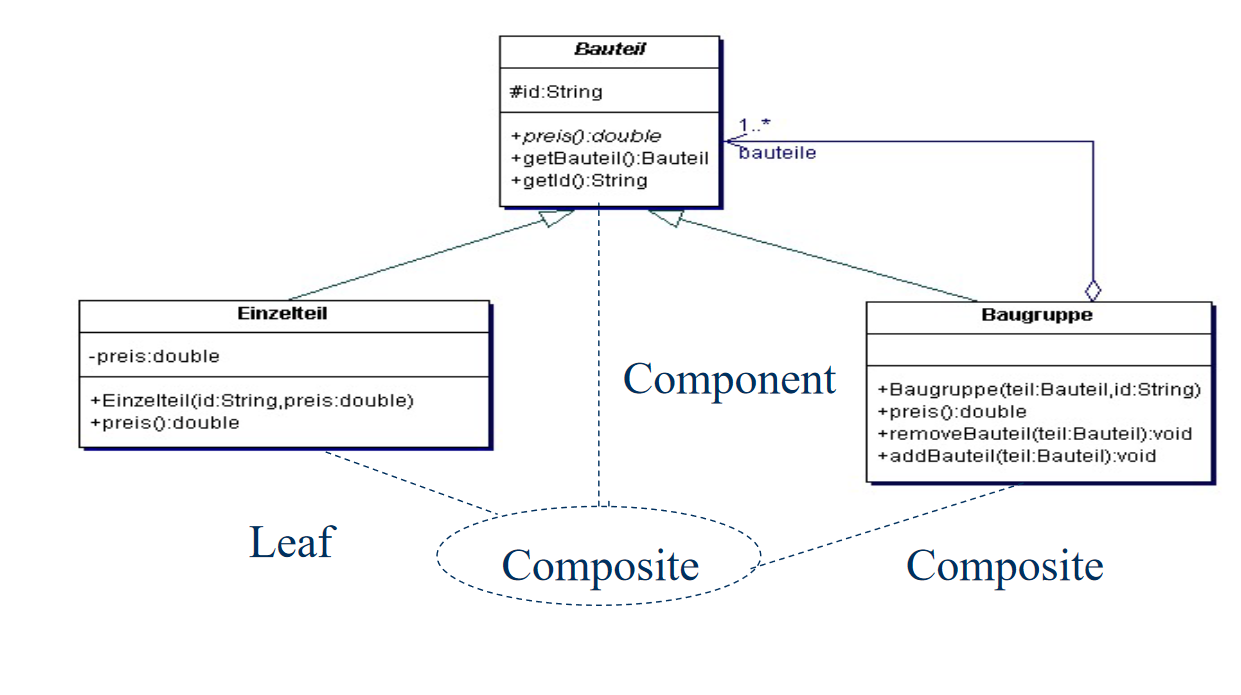
\includegraphics[width=0.75\textwidth]{aufgabe1}
		\end{center}
		\item Datei \texttt{Bauteil.java}
		\begin{lstlisting}[style=java, tabsize=2]
public abstract class Bauteil {
	protected String id;

	public abstract double preis();

	public String getId() {
		return id;
	}
}
		\end{lstlisting}
		Datei \texttt{Einzelteil.java}
		\begin{lstlisting}[style=java, tabsize=2]
public class Einzelteil extends Bauteil {
	private double preis;

	public Einzelteil(String id, double preis) {
		this.preis = preis;
		this.id = id;
	}

	@Override
	public double preis() {
		return preis;
	}
}
		\end{lstlisting}
		Datei \texttt{Baugruppe.java}, gleich mit Verbesserungen
		\begin{lstlisting}[style=java, tabsize=2]
import java.util.Set;

public class Baugruppe extends Bauteil {
	private Set<Bauteil> bauteile;

	public Baugruppe (Bauteil teil, String id){
		if(teil != null){
			this.bauteile = new HashSet<Bauteil>();
			this.id = id;
		} else {
			throw new Exception("Gib mir ein Bauteil !11!!11!1");
		}
	}

	public double preis() {
		double summe = 0;
		for (Bauteil b : bauteile) {
			summe += b.preis();
		}
		return summe;
	}

	// void Rueckgabe ist nicht so gut
	// keine Info ueber Miss-/Erfolg des Loeschens
	// void -> boolean
	// Problem: was ist mit Bauteilen, die in Baugruppen
	// versteckt sind? auch mit entfernen oder nicht? -> nur 1 
	// Ebene betrachten
	// keine Rekursion
	public boolean removeBauteil(Bauteil teil){
		if (bauteile.size() == 1) {
			return false;
		} else {
			return bauteile.remove(teil);
		}
	}

	// void Rueckgabe ist nicht so gut
	// keine Info ueber Miss-/Erfolg des Einfuegens
	// + man erfaehrt nicht, ob Duplikat vorlag
	// void -> boolean

	// Refaktorisierte, Set-basierte Variante ohne Exception
	// Ausnahmebehandlung sollte man nicht zur Behandlung 
	// normaler (d.h. haeufig auftretender) Programmsituationen 
	// einsetzen.
	// (Siehe auch Tipp 34 aus "The Pragmatic Programmer": 
	// "Use Exceptions for Exceptional Problems" und Item 57 
	// aus "Effective Java": "Use exceptions only for 
	// exceptional conditions".)
	public boolean addBauteil(Bauteil teil){
		return bauteile.add(teil);
	}
}
		\end{lstlisting}
		\item  Im Set würde das \texttt{t4} abgelehnt, in der Liste nicht.
	\end{enumerate}

	\section*{Aufgabe 2}
	\begin{enumerate}[label=(\alph*)]
		\item UML-Diagramm
		\begin{center}
			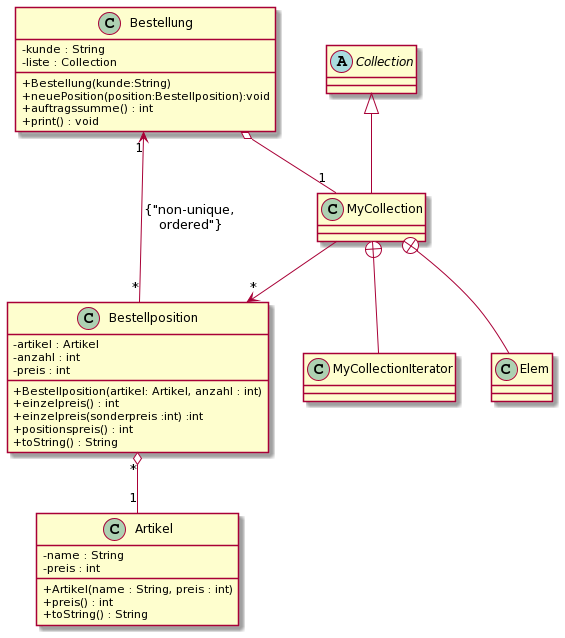
\includegraphics[width=0.70\textwidth]{aufgabe2a}
		\end{center}
		\item UML-Diagramm mit Iterator-Pattern
		\begin{center}
			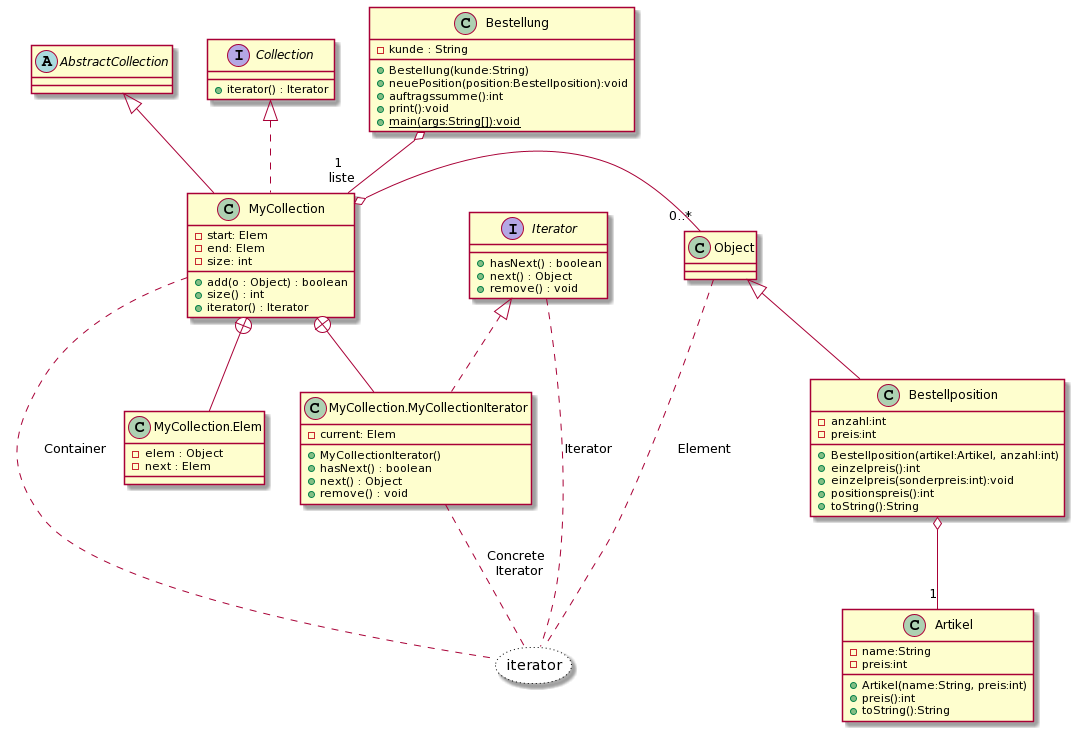
\includegraphics[width=1\textwidth]{aufgabe2b}
		\end{center}
		\item Datei \texttt{Bestellung.java}
		\begin{lstlisting}[style=java, tabsize=2]
import java.util.Collection;
import java.util.Iterator;

public class Bestellung {
	private String kunde;
	private Collection<Bestellposition> liste;

	public Bestellung(String kunde) {
		this.kunde = kunde;
		liste = new MyCollection<Bestellposition>();
	}

	public void neuePosition(Bestellposition position) {
		liste.add(position);
	}

	public int auftragssumme() {
		Iterator iter = liste.iterator();
		int summe = 0;
		while (iter.hasNext()) {
			summe += iter.next().positionspreis();
		}
		return summe;
	}

	public void print() {
		System.out.println("Bestellung fuer Kunde " + kunde);
		Iterator iter = liste.iterator();
		int pos = 0;
		while (iter.hasNext()) {
			System.out.println(pos + ". " + iter.next());
			pos++;
		}
		System.out.println("Auftragssumme: " + auftragssumme());
		System.out.println();
	}

	public static void main(String[] args) {
		Artikel tisch = new Artikel("Tisch", 200);
		Artikel stuhl = new Artikel("Stuhl", 100);
		Artikel schrank = new Artikel("Schrank", 300);

		Bestellung bestellung = new Bestellung("TUD");
		bestellung.neuePosition(new Bestellposition(tisch, 1));
		bestellung.neuePosition(new Bestellposition(stuhl, 4));
		bestellung.neuePosition(new Bestellposition(schrank, 2));
		bestellung.print();
	}
}
		\end{lstlisting}
		Datei \texttt{MyCollection.java}
		\begin{lstlisting}[style=java,tabsize=2]
import java.util.AbstractCollection;
import java.util.Collection;
import java.util.Iterator;

public class MyCollection<T> extends AbstractCollection<T> implements Collection<T> {
	private class Elem {
		private T elem;
		private Elem next;

		public Elem(T elem, Elem next) {
			this.elem = elem;
			this.next = next;
		}
	}

	private Elem start = null;
	private Elem end = null;
	private int size = 0;

	@Override
	public boolean add(T o) {
		Elem e = new Elem(o, null);
		if (end != null) {
			end.next = e;
		}
		if (start == null) {
			start = e;
		}
		end = e;
		size++;
		return true;
	}

	@Override
	public int size() {
		return size;
	}

	private class MyCollectionIterator implements Iterator<T> {
		private Elem current;

		public MyCollectionIterator() {
			current = start;
		}

		@Override
		public boolean hasNext() {
			return current != null;
		}

		@Override
		public T next() {
			T o = current.elem;
			current = current.next;
			return o;
		}

		@Override
		public void remove() {
			throw new UnsupportedOperationException("Keine Lust zur Implementation");
		}
	}

	@Override
	public Iterator iterator() {
		return new MyCollectionIterator();
	}
}
		\end{lstlisting}
	\end{enumerate}
	
\end{document}